% Gabarit pandoc des corrigés publiés (brut et guidé). Contenu sans marque ni nom de site.
% Compilation : lualatex (latexmk -lualatex).
% Le Markdown reste la source unique : ne pas éditer ce fichier .tex à la main.
\documentclass[11pt,a4paper]{article}

% --- Moteur, polices (Latin Modern) et langue ---------------------------------
\usepackage{iftex}
\ifLuaTeX\else\errmessage{Ce document se compile avec lualatex}\fi
\usepackage{amsmath,amssymb,mathtools}
\usepackage{fontspec}
% mathrm=sym : \mathrm prend ses glyphes dans la police mathématique (ℓ, μ, Ω), comme KaTeX.
\usepackage[math-style=TeX,bold-style=TeX,mathrm=sym]{unicode-math}
% Repli pour les glyphes absents de Latin Modern (indices et exposants Unicode,
% flèches, filets des schémas en texte, symboles) : DejaVu, puis Latin Modern Math
% (ℓ, lettres mathématiques Unicode des légendes).
\directlua{
  luaotfload.add_fallback("repliTexte", {"DejaVuSerif:mode=harf;", "DejaVuSans:mode=harf;", "file:latinmodern-math.otf:mode=harf;"})
  luaotfload.add_fallback("repliMono", {"DejaVuSansMono:mode=harf;", "DejaVuSans:mode=harf;", "file:latinmodern-math.otf:mode=harf;"})
}
\setmainfont{Latin Modern Roman}[RawFeature={fallback=repliTexte}]
\setsansfont{Latin Modern Sans}[RawFeature={fallback=repliTexte}]
\setmonofont{Latin Modern Mono}[RawFeature={fallback=repliMono}]
\setmathfont{Latin Modern Math}
\usepackage[french]{babel}
\frenchsetup{SmallCapsFigTabCaptions=false}

% --- Mise en page --------------------------------------------------------------
\usepackage[a4paper,margin=2.2cm,headheight=14pt,footskip=1.2cm]{geometry}
\usepackage{microtype}
\setlength{\emergencystretch}{4em}
\tolerance=1500
\setlength{\parindent}{0pt}
\setlength{\parskip}{0.55\baselineskip plus 2pt minus 1pt}
\usepackage{xcolor}
% Gris nommés : babel-french rend « ! » actif dans le document.
\definecolor{gris2}{gray}{0.98}
\definecolor{gris3}{gray}{0.97}
\definecolor{gris5}{gray}{0.95}
\definecolor{gris35}{gray}{0.65}
\definecolor{gris40}{gray}{0.60}
\definecolor{gris45}{gray}{0.55}
\definecolor{gris50}{gray}{0.50}
\definecolor{gris55}{gray}{0.45}
\definecolor{gris60}{gray}{0.40}
\definecolor{gris65}{gray}{0.35}
\definecolor{gris70}{gray}{0.30}
\definecolor{gris80}{gray}{0.20}
\definecolor{gris85}{gray}{0.15}
\usepackage{graphicx}
\usepackage{float}
\usepackage{caption}
\captionsetup{font=small,labelformat=empty,justification=centering}
\usepackage{booktabs,longtable,array,multirow,calc}
\usepackage{siunitx}
\sisetup{locale=FR}
\usepackage[version=4]{mhchem}
\usepackage{listings}
\usepackage{fancyhdr}
\usepackage{lastpage}
\usepackage[most]{tcolorbox}
\usepackage{enumitem}
\setlist{nosep,leftmargin=*,topsep=2pt}
\usepackage[hidelinks,unicode]{hyperref}
\usepackage{bookmark}
\hypersetup{pdftitle={Centrale-Supélec MP — Physique-chimie 1 2026},pdfauthor={Rédigé par IA},pdfcreator={LaTeX},pdfsubject={Corrigé brut}}
\usepackage{xurl}

% --- Pandoc : listes, tableaux, figures ----------------------------------------
\providecommand{\passthrough}[1]{#1}
\providecommand{\tightlist}{\setlength{\itemsep}{0pt}\setlength{\parskip}{0pt}}

\makeatletter
\def\maxwidth{\ifdim\Gin@nat@width>\linewidth\linewidth\else\Gin@nat@width\fi}
\def\maxheight{\ifdim\Gin@nat@height>0.55\textheight 0.55\textheight\else\Gin@nat@height\fi}
\makeatother
\setkeys{Gin}{width=\maxwidth,height=\maxheight,keepaspectratio}
\setcounter{secnumdepth}{-\maxdimen}
\providecommand{\pandocbounded}[1]{#1}
\usepackage{longtable,booktabs,array}

% --- Code (listings) -----------------------------------------------------------
\lstset{
  basicstyle=\ttfamily\small,
  columns=fullflexible,
  keepspaces=true,
  breaklines=true,
  breakatwhitespace=false,
  postbreak=\mbox{\textcolor{gris50}{$\hookrightarrow$}\space},
  frame=single,
  rulecolor=\color{gris35},
  framesep=4pt,
  xleftmargin=5pt,xrightmargin=5pt,
  backgroundcolor=\color{gris3},
  keywordstyle=\bfseries,
  commentstyle=\color{gris65},
  stringstyle=\color{gris80},
  showstringspaces=false,
  tabsize=4,
  extendedchars=true,
  aboveskip=6pt,belowskip=6pt,
}

% --- Macros des corrigés (KaTeX ↔ LaTeX) ---------------------------------------
% Les corrigés sont écrits pour KaTeX : on définit ici ce que KaTeX connaît et
% que LaTeX n'a pas, sans jamais retoucher le Markdown.
\providecommand{\R}{\mathbb{R}}
\providecommand{\N}{\mathbb{N}}
\providecommand{\Z}{\mathbb{Z}}
\providecommand{\Q}{\mathbb{Q}}
\providecommand{\C}{\mathbb{C}}
\providecommand{\dd}{\mathrm{d}}
\providecommand{\llbracket}{\lBrack}
\providecommand{\rrbracket}{\rBrack}
\providecommand{\lBrace}{\lbrace}
\providecommand{\rBrace}{\rbrace}
\providecommand{\Box}{\square}
\providecommand{\Diamond}{\lozenge}
\providecommand{\varnothing}{\emptyset}
\providecommand{\argmax}{\operatorname*{arg\,max}}
\providecommand{\argmin}{\operatorname*{arg\,min}}
\renewcommand{\leq}{\leqslant}
\renewcommand{\geq}{\geqslant}

% Équation hors texte : réduite à la largeur de la ligne si elle déborde.
\newsavebox{\boiteequation}
\newcommand{\equationajustee}[1]{%
  \sbox{\boiteequation}{$\displaystyle #1$}%
  \ifdim\wd\boiteequation>\linewidth
    \[\resizebox{\linewidth}{!}{\usebox{\boiteequation}}\]%
  \else
    \[#1\]%
  \fi}

% --- Encadrés pédagogiques (sobres, lisibles en noir et blanc) -----------------
\tcbset{
  encadre/.style={
    enhanced,breakable,sharp corners,
    colback=white,colframe=gris55,
    boxrule=0.4pt,leftrule=2.2pt,
    left=6pt,right=6pt,top=3pt,bottom=3pt,
    before skip=6pt,after skip=6pt,
    fonttitle=\bfseries\small,coltitle=black,
    attach title to upper,after title={\quad},
    parbox=false,
  }
}
\newtcolorbox{indication}[1]{encadre,colframe=gris45,colback=gris2,title={Indication~#1}}
\newtcolorbox{methode}{encadre,colframe=gris70,title={Méthode}}
\newtcolorbox{piege}{encadre,colframe=gris85,boxrule=0.8pt,leftrule=2.2pt,title={Piège}}
\newtcolorbox{jury}{encadre,colframe=gris60,colback=gris5,title={Jury}}
\newtcolorbox{encadrenote}{encadre,colframe=gris40}

% --- Titres de section ---------------------------------------------------------
\usepackage{titlesec}
\titleformat{\section}{\Large\bfseries}{}{0pt}{}
\titleformat{\subsection}{\large\bfseries}{}{0pt}{}
\titleformat{\subsubsection}{\normalsize\bfseries}{}{0pt}{}
\titlespacing*{\section}{0pt}{14pt plus 4pt minus 2pt}{6pt}
\titlespacing*{\subsection}{0pt}{10pt plus 3pt minus 2pt}{4pt}
\titlespacing*{\subsubsection}{0pt}{8pt plus 2pt minus 2pt}{2pt}

% --- En-tête et pied de page ---------------------------------------------------
\pagestyle{fancy}
\fancyhf{}
\fancyhead[L]{\small\textsc{Corrigé brut} · Centrale-Supélec MP}
\fancyhead[R]{\small Physique-chimie 1 2026}
\fancyfoot[L]{\footnotesize Corrigé rédigé par IA, non officiel}
\fancyfoot[R]{\footnotesize \thepage\,/\,\pageref*{LastPage}}
\renewcommand{\headrulewidth}{0.4pt}
\renewcommand{\footrulewidth}{0pt}
\fancypagestyle{plain}{\fancyhf{}\fancyfoot[R]{\footnotesize \thepage\,/\,\pageref*{LastPage}}\fancyfoot[L]{\footnotesize Corrigé rédigé par IA, non officiel}\renewcommand{\headrulewidth}{0pt}}

\begin{document}
\thispagestyle{plain}
\begin{center}
  {\small\scshape Corrigé brut}\par\smallskip
  {\LARGE\bfseries Centrale-Supélec MP — Physique-chimie 1 2026\par}\medskip
  {\large Centrale-Supélec · MP · Physique-chimie 1 · 2026\par}
\end{center}
\vspace{2pt}\hrule\vspace{8pt}

\emph{Corrigé rédigé par IA, non officiel. Signalez toute erreur.}

Épreuve de 4 heures, calculatrice autorisée. « Spectroscopie rovibrationnelle et laser » : 46 questions. Constantes utilisées :

\begin{itemize}
\tightlist
\item
  \(h=6{,}626\times10^{-34}\) J·s et \(\hbar=1{,}0546\times10^{-34}\) J·s ;
\item
  \(c=2{,}998\times10^{8}\) m·s⁻¹ ;
\item
  \(1\ \mathrm{cm^{-1}}\leftrightarrow1{,}9863\times10^{-23}\ \mathrm J\) ;
\item
  \(m_{\mathrm H}=1{,}66\times10^{-27}\) kg ;
\item
  en Q12, la constante de Boltzmann \(k_B=1{,}38\times10^{-23}\) J·K⁻¹ (non fournie).
\end{itemize}

\hypertarget{partie-a-spectroscopie-rovibrationnelle}{%
\section{Partie A --- Spectroscopie rovibrationnelle}\label{partie-a-spectroscopie-rovibrationnelle}}

\hypertarget{i-vibration-de-hcl}{%
\subsection{I --- Vibration de HCl}\label{i-vibration-de-hcl}}

\textbf{Q1.} La force de rappel vaut \(F_x=-\dfrac{\mathrm dE_p}{\mathrm dx}=-\mu\omega_0^2x\). Le principe fondamental de la dynamique, projeté sur \((Ox)\) dans un référentiel galiléen, donne

\equationajustee{\boxed{\ddot x+\omega_0^2x=0}}

L'équation caractéristique \(r^2+\omega_0^2=0\) a pour racines \(\pm j\omega_0\) ; la solution générale réelle est

\equationajustee{\boxed{\begin{aligned}
x(t)&=A\cos(\omega_0t)+B\sin(\omega_0t)\\
&=X_m\cos(\omega_0t+\varphi)
\end{aligned}}}

avec \((A,B)\) ou \((X_m,\varphi)\) fixées par les conditions initiales.

\textbf{Q2.} Avec \(x=X_m\cos(\omega_0t+\varphi)\) et la référence \(E_p(0)=0\) :

\equationajustee{\begin{aligned}
E_c&=\frac12\mu\omega_0^2X_m^2\sin^2(\omega_0t+\varphi)\\
E_p&=\frac12\mu\omega_0^2X_m^2\cos^2(\omega_0t+\varphi)
\end{aligned}}

Les moyennes sur une période valent

\equationajustee{\begin{aligned}
\langle E_c\rangle&=\tfrac14\mu\omega_0^2X_m^2\\
\langle E_p\rangle&=\tfrac14\mu\omega_0^2X_m^2\\
\langle E_m\rangle&=\tfrac12\mu\omega_0^2X_m^2
\end{aligned}}

Elles sont positives ou nulles et s'annulent simultanément pour \(X_m=0\). La particule immobile en \(x=0\) est une solution permise (\(x(0)=0\), \(\dot x(0)=0\)). Donc \textbf{les trois minima valent 0 et sont atteints} (oscillateur au repos au fond du puits).

\textbf{Q3.} Dans un état stationnaire lié, \(\lvert\Psi\rvert^2=\lvert\varphi(x)\rvert^2\) ne dépend pas du temps et \(\varphi\to0\) à l'infini.

\emph{Position.} \(E_p\) est paire. Si \(\varphi(x)\) est solution d'énergie \(E\), \(\varphi(-x)\) l'est aussi.

Les états liés à une dimension étant non dégénérés, \(\varphi(-x)=\pm\varphi(x)\). La densité \(\lvert\varphi\rvert^2\) est donc paire, d'où

\equationajustee{\begin{aligned}
\langle x\rangle&=\int x\lvert\varphi\rvert^2\,\mathrm dx=0\\
\Delta x^2&=\langle x^2\rangle
\end{aligned}}

\emph{Quantité de mouvement.} L'équation de Schrödinger stationnaire étant à coefficients réels, on peut prendre \(\varphi\) réelle. Alors

\equationajustee{\begin{aligned}
\langle p_x\rangle&=-j\hbar\int\varphi\varphi'\,\mathrm dx\\
&=-j\hbar\left[\varphi^2/2\right]_{-\infty}^{+\infty}\\
&=0
\end{aligned}}

donc \(\Delta p_x^2=\langle p_x^2\rangle\).

Par suite :

\equationajustee{\begin{aligned}
\langle E_p\rangle&=\frac12\mu\omega_0^2\langle x^2\rangle\\
&=\frac12\mu\omega_0^2\Delta x^2\\
\langle E_c\rangle&=\frac{\langle p_x^2\rangle}{2\mu}\\
&=\frac{\Delta p_x^2}{2\mu}
\end{aligned}}

\equationajustee{\boxed{\begin{aligned}
K_1&=\tfrac12\mu\omega_0^2\\
K_2&=\frac{1}{2\mu}
\end{aligned}}}

\textbf{Q4.} D'après Q3 :

\equationajustee{\langle E_m\rangle=\frac{\Delta p_x^2}{2\mu}+\frac12\mu\omega_0^2\Delta x^2}

L'inégalité de Heisenberg \(\Delta x\,\Delta p_x\ge\hbar/2\) (avec \(\Delta x>0\)) donne \(\Delta p_x^2\ge\hbar^2/(4\Delta x^2)\). Avec l'inégalité \(a+b\ge2\sqrt{ab}\), il vient

\equationajustee{\begin{aligned}
\langle E_m\rangle&\ge\frac{\hbar^2}{8\mu\Delta x^2}+\frac12\mu\omega_0^2\Delta x^2\\
&\ge2\sqrt{\frac{\hbar^2}{8\mu}\cdot\frac{\mu\omega_0^2}{2}}\\
&=\frac{\hbar\omega_0}{2}
\end{aligned}}

l'égalité ayant lieu pour \(\Delta x^2=\hbar/(2\mu\omega_0)\) :

\equationajustee{\boxed{\langle E_m\rangle_{\min}=\frac{\hbar\omega_0}{2}}}

Classiquement le minimum est nul (repos au fond du puits). Quantiquement, annuler \(\langle E_p\rangle\) exigerait \(\Delta x=0\), donc \(\Delta p_x\) infini. L'oscillateur ne peut pas être immobile : il garde une \textbf{énergie de point zéro} \(\hbar\omega_0/2\), atteinte par le niveau fondamental (Q8).

\textbf{Q5.} Les dimensions sont \([\hbar]=\mathrm{M\,L^2\,T^{-1}}\), \([\omega_0]=\mathrm T^{-1}\) et \([\mu]=\mathrm M\). L'égalité \([a_0]=\mathrm L\) impose, sur M, L et T :

\equationajustee{\begin{aligned}
\alpha+\delta&=0\\
2\alpha&=1\\
-\alpha-\beta&=0
\end{aligned}}

\equationajustee{\boxed{\begin{aligned}
\alpha&=\tfrac12\\
\beta&=-\tfrac12\\
\delta&=-\tfrac12
\end{aligned}}}

\equationajustee{\boxed{a_0=\sqrt{\frac{\hbar}{\mu\omega_0}}}}

Avec \(\mu\simeq m_{\mathrm H}\) et \(\omega_0\simeq10^{15}\) rad·s⁻¹ :

\equationajustee{a_0=\sqrt{\frac{1{,}05\times10^{-34}}{1{,}66\times10^{-27}\times10^{15}}}}

soit

\equationajustee{\boxed{a_0\approx8\times10^{-12}\ \mathrm m\sim10^{-11}\ \mathrm m}}

C'est quelques pour cent de la longueur de liaison (\(\sim10^{-10}\) m) : les oscillations sont petites, ce qui justifie le modèle harmonique.

\textbf{Q6.} Pour un état stationnaire d'énergie \(E\), la séparation des variables dans \(j\hbar\,\partial_t\Psi=\hat H\Psi\) donne

\equationajustee{\boxed{\chi(t)=\chi_0\,e^{-jEt/\hbar}}}

La partie spatiale vérifie

\equationajustee{-\frac{\hbar^2}{2\mu}\frac{\mathrm d^2\varphi}{\mathrm dx^2}+\frac12\mu\omega_0^2x^2\varphi=E\varphi}

On pose \(x=a_0u\), avec \(a_0^2=\hbar/(\mu\omega_0)\). Les deux préfacteurs deviennent

\equationajustee{\begin{aligned}
\frac{\hbar^2}{2\mu a_0^2}&=\frac{\hbar\omega_0}{2}\\
\frac12\mu\omega_0^2a_0^2&=\frac{\hbar\omega_0}{2}
\end{aligned}}

En divisant par \(\hbar\omega_0\) :

\equationajustee{\boxed{\varphi''(u)+\left(2\varepsilon-u^2\right)\varphi(u)=0}}

\textbf{Q7.} Avec \(\varphi=\mathcal H e^{-u^2/2}\) :

\equationajustee{\begin{aligned}
\varphi'&=(\mathcal H'-u\mathcal H)e^{-u^2/2}\\
\varphi''&=\left(\mathcal H''-2u\mathcal H'+(u^2-1)\mathcal H\right)e^{-u^2/2}
\end{aligned}}

En reportant et en simplifiant par \(e^{-u^2/2}\neq0\), les termes en \(u^2\mathcal H\) se compensent :

\equationajustee{\boxed{\mathcal H''(u)-2u\,\mathcal H'(u)+(2\varepsilon-1)\,\mathcal H(u)=0}}

\textbf{Q8.} \(\mathcal H''\) est de degré \(n-2\) et ne contribue pas au coefficient de \(u^n\).

Ce coefficient vaut \(-2nc_n\) dans \(-2u\mathcal H'\), et \((2\varepsilon-1)c_n\) dans \((2\varepsilon-1)\mathcal H\).

Le polynôme étant nul et \(c_n\neq0\) :

\equationajustee{-2n+2\varepsilon-1=0}

\equationajustee{\boxed{\varepsilon=n+\tfrac12}}

Les énergies de vibration en découlent :

\equationajustee{\boxed{E_n=\left(n+\tfrac12\right)\hbar\omega_0,\quad n\in\mathbb N}}

Les niveaux sont équidistants de \(\hbar\omega_0\) et le fondamental vaut \(\hbar\omega_0/2\), borne de Q4.

\begin{figure}[H]
\centering
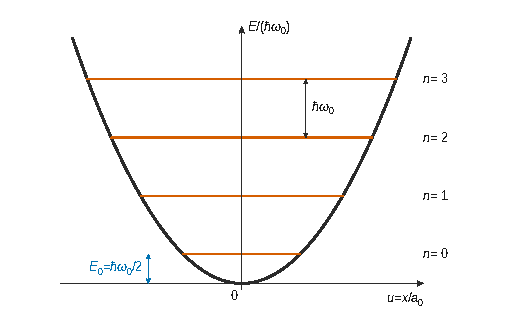
\includegraphics{figures/q8-niveaux-oscillateur.pdf}
\caption*{Figure 1 --- Puits harmonique et niveaux E\_n = (n + ½)ħω₀ : niveaux
équidistants de ħω₀, fondamental à l'énergie de point zéro ħω₀/2}
\end{figure}

\hypertarget{ii-rovibration-de-hcl}{%
\subsection{II --- Rovibration de HCl}\label{ii-rovibration-de-hcl}}

\textbf{Q9.}

\equationajustee{\begin{aligned}
\Delta E_J&=B\left[(J+1)(J+2)-J(J+1)\right]\\
&=\boxed{2B(J+1)}
\end{aligned}}

\textbf{Q10.} On considère une transition \((n=0,J'')\to(n=1,J')\), avec la même constante \(B\) pour les deux états. On note \(\tilde B=B/(hc)\) et \(\tilde\nu_0=\omega_0/(2\pi c)\) :

\begin{itemize}
\tightlist
\item
  branche R (\(J'=J''+1\)) : \(\tilde\nu=\tilde\nu_0+2\tilde B(J''+1)>\tilde\nu_0\) ;
\item
  branche P (\(J'=J''-1\), \(J''\ge1\)) : \(\tilde\nu=\tilde\nu_0-2\tilde BJ''<\tilde\nu_0\).
\end{itemize}

Sur la figure 3 (axe des nombres d'onde \textbf{décroissant} vers la droite), les raies sont espacées d'environ 20 cm⁻¹, sauf entre 2865 et 2906 cm⁻¹. Cet écart de 41 cm⁻¹, soit \(4\tilde B\), est dû à l'absence de transition \(\Delta J=0\) : c'est le centre de bande, \(\tilde\nu_0\approx2886\) cm⁻¹. D'où

\equationajustee{\boxed{\begin{aligned}{}&\text{branche R : }[2886\,;3100]\ \mathrm{cm^{-1}}\ (\text{raies de 2906 \text{à} 3073})\\
&\text{branche P : }[2600\,;2886]\ \mathrm{cm^{-1}}\ (\text{raies de 2626 \text{à} 2865})
\end{aligned}}}

La branche R est à gauche de la figure, la branche P à droite.

\begin{figure}[H]
\centering
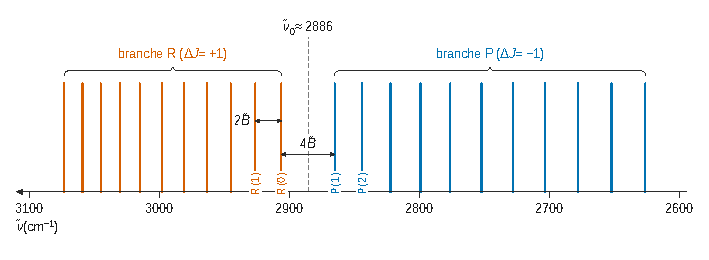
\includegraphics{figures/q10-branches-p-r.pdf}
\caption*{Figure 2 --- Lecture de la figure 3 (axe décroissant) : branche R à
gauche, branche P à droite, trou central de 4B̃ autour de ν̃₀ ≈ 2886 cm⁻¹,
attribution de R(0), R(1), P(1) et P(2)}
\end{figure}

\textbf{Q11.} En partant du trou central : la première raie R est R(0), la première raie P est P(1) (pas de P(0), car \(J'=-1\) n'existe pas).

\begin{longtable}[]{@{}llll@{}}
\toprule\noalign{}
\(\tilde\nu\) (cm⁻¹) & \(J''\) & \(J'\) & branche \\
\midrule\noalign{}
\endhead
\bottomrule\noalign{}
\endlastfoot
2926 & 1 & 2 & R \\
2906 & 0 & 1 & R \\
2865 & 1 & 0 & P \\
2844 & 2 & 1 & P \\
\end{longtable}

Contrôle avec \(\tilde\nu_0=2885{,}5\) cm⁻¹ et \(\tilde B=10{,}25\) cm⁻¹ (Q13) : on trouve 2906 ; 2926,5 ; 2865 et 2844,5 cm⁻¹, conformes à 1 cm⁻¹ près.

\textbf{Q12.} Deux raisons.

\emph{Transitions possibles.} Les raies de la bande \(n=0\to n=1\) sont en \(\tilde\nu_0+2\tilde B(J''+1)\) et \(\tilde\nu_0-2\tilde BJ''\) : plus \(J''\) est grand, plus elles s'écartent du centre.

Les autres transitions tombent loin de la fenêtre. La rotation pure est à quelques dizaines de cm⁻¹ (infrarouge lointain). La bande \(n=0\to2\) est vers \(2\tilde\nu_0\approx5800\) cm⁻¹ (et quasi interdite dans le modèle harmonique).

\emph{Population des niveaux de départ.} L'intensité d'une raie d'absorption est proportionnelle à la population du niveau \(J''\). Celle-ci est pondérée par le facteur de Boltzmann \(\exp\left(-\tilde BJ''(J''+1)\,hc/k_BT\right)\). À 300 K :

\equationajustee{\frac{k_BT}{hc}=\frac{1{,}38\times10^{-23}\times300}{1{,}9863\times10^{-23}}\approx208\ \mathrm{cm^{-1}}}

Le facteur vaut alors \(4\times10^{-3}\) pour \(J''=10\). Il tombe à \(5\times10^{-4}\) pour \(J''=12\).

Les raies au-delà de \(J''\approx11\text{–}12\) sont situées hors de \(\tilde\nu_0\pm2\tilde B\times12\approx2886\pm250\) cm⁻¹. Elles partent donc de niveaux quasi vides : \textbf{il n'y a pas de transition permise issue d'un niveau thermiquement peuplé en dehors de \([2600\,;3100]\) cm⁻¹.} La dégénérescence \(2J+1\) des niveaux de rotation explique que le maximum d'intensité soit vers \(J''\approx3\) ; elle ne change pas cette conclusion.

\textbf{Q13.} \emph{Démarche.} Le modèle comporte deux inconnues, \(\tilde\nu_0\) et \(\tilde B\). Les deux raies qui encadrent le trou, R(0) et P(1), donnent directement leur somme et leur différence. Ce sont aussi les moins sensibles à l'écart entre les constantes rotationnelles des deux états (petits \(J\)) :

\equationajustee{\begin{aligned}
\text{R(0)}:\quad\tilde\nu_0+2\tilde B&=2906\ \mathrm{cm^{-1}}\\
\text{P(1)}:\quad\tilde\nu_0-2\tilde B&=2865\ \mathrm{cm^{-1}}
\end{aligned}}

\equationajustee{\begin{aligned}
\tilde\nu_0&=\frac{2906+2865}{2}\\
&=2885{,}5\ \mathrm{cm^{-1}}\\
\tilde B&=\frac{2906-2865}{4}\\
&=10{,}25\ \mathrm{cm^{-1}}
\end{aligned}}

Les deux lectures sont indépendantes, d'incertitude-type 1 cm⁻¹. On obtient \(u(\tilde\nu_0)=\frac{\sqrt2}{2}=0{,}71\) cm⁻¹ et \(u(\tilde B)=\frac{\sqrt2}{4}=0{,}35\) cm⁻¹.

\emph{Longueur \(d_0\).} La constante rotationnelle vaut

\equationajustee{\begin{aligned}
B&=hc\tilde B\\
&=10{,}25\times1{,}9863\times10^{-23}\\
&=2{,}036\times10^{-22}\ \mathrm J
\end{aligned}}

La masse réduite de \(\mathrm H^{35}\mathrm{Cl}\) (isotope majoritaire) vaut \(\mu=\frac{35}{36}m_{\mathrm H}=1{,}614\times10^{-27}\) kg. De \(B=\hbar^2/(2\mu d_0^2)\) :

\equationajustee{\begin{aligned}
d_0&=\frac{\hbar}{\sqrt{2\mu B}}\\
&=\frac{1{,}0546\times10^{-34}}{\sqrt{2\times1{,}614\times10^{-27}\times2{,}036\times10^{-22}}}\\
&=1{,}30\times10^{-10}\ \mathrm m
\end{aligned}}

Comme \(d_0\propto\tilde B^{-1/2}\), \(u(d_0)/d_0=\frac12u(\tilde B)/\tilde B=1{,}7\) \% :

\equationajustee{\boxed{d_0=(1{,}30\pm0{,}02)\times10^{-10}\ \mathrm m}}

\emph{Pulsation \(\omega_0\).} Le centre de bande correspond à \(\hbar\omega_0=hc\tilde\nu_0\) :

\equationajustee{\begin{aligned}
\omega_0&=2\pi c\tilde\nu_0\\
&=\frac{2885{,}5\times1{,}9863\times10^{-23}}{1{,}0546\times10^{-34}}\\
&=5{,}435\times10^{14}\ \mathrm{rad\cdot s^{-1}}
\end{aligned}}

\equationajustee{\begin{aligned}
u(\omega_0)&=\omega_0\frac{u(\tilde\nu_0)}{\tilde\nu_0}\\
&=1{,}3\times10^{11}\ \mathrm{rad\cdot s^{-1}}
\end{aligned}}

\equationajustee{\boxed{\begin{aligned}
\omega_0&=5{,}435\times10^{14}\ \mathrm{rad\cdot s^{-1}}\\
u(\omega_0)&=1{,}3\times10^{11}\ \mathrm{rad\cdot s^{-1}}
\end{aligned}}}

\emph{Contrôles.} \(d_0\sim10^{-10}\) m et \(\omega_0\sim5\times10^{14}\) rad·s⁻¹ sont cohérents avec l'énoncé et avec Q5.

L'hypothèse d'une même constante rotationnelle n'est qu'approchée. Les espacements décroissent dans la branche R (20 à 14 cm⁻¹) et croissent dans la branche P (21 à 26 cm⁻¹), signe que \(\tilde B'<\tilde B''\). Les différences de combinaison, indépendantes de l'état excité, s'écrivent

\equationajustee{\tilde\nu_{\mathrm R(J-1)}-\tilde\nu_{\mathrm P(J+1)}=2\tilde B''(2J+1)}

Elles donnent \(\tilde B''\approx10{,}35\) cm⁻¹ et \(d_0\approx1{,}29\times10^{-10}\) m, compatible avec le résultat ci-dessus.

\textbf{Q14.} Le chlore naturel contient \(^{35}\)Cl (76 \%) et \(^{37}\)Cl (24 \%) ; l'hydrogène est pratiquement pur (\(^1\)H à 99,985 \%). Les molécules \(\mathrm H^{35}\mathrm{Cl}\) et \(\mathrm H^{37}\mathrm{Cl}\) ont la même liaison (même raideur) mais des masses réduites différentes :

\equationajustee{\begin{aligned}
\frac{\mu_{37}}{\mu_{35}}&=\frac{37\times36}{38\times35}\\
&=1{,}0015
\end{aligned}}

Comme \(\omega_0\propto\mu^{-1/2}\) :

\equationajustee{\begin{aligned}
\frac{\Delta\tilde\nu_0}{\tilde\nu_0}&=\sqrt{\frac{\mu_{35}}{\mu_{37}}}-1\\
&=-7{,}5\times10^{-4}\\
\Delta\tilde\nu_0&\approx-2{,}2\ \mathrm{cm^{-1}}
\end{aligned}}

(\(\tilde B\propto1/\mu\) varie aussi, effet secondaire.) \textbf{Chaque raie est un doublet isotopique : la raie de \(\mathrm H^{35}\mathrm{Cl}\) est accompagnée, environ 2 cm⁻¹ plus bas, de celle de \(\mathrm H^{37}\mathrm{Cl}\), environ trois fois moins intense (76/24).}

\hypertarget{partie-b-cavituxe9-dun-laser}{%
\section{Partie B --- Cavité d'un laser}\label{partie-b-cavituxe9-dun-laser}}

\hypertarget{i-cavituxe9-sans-pertes}{%
\subsection{I --- Cavité sans pertes}\label{i-cavituxe9-sans-pertes}}

\textbf{Q15.} Dans le vide (\(\rho=0\), \(\vec\jmath=\vec0\)) :

\equationajustee{\boxed{\begin{aligned}{}&\mathrm{div}\,\vec E=0 &&\text{(Maxwell-Gauss)}\\
&\mathrm{div}\,\vec B=0 &&\text{(Maxwell-flux)}\\
&\overrightarrow{\mathrm{rot}}\,\vec E=-\frac{\partial\vec B}{\partial t} &&\text{(Maxwell-Faraday)}\\
&\overrightarrow{\mathrm{rot}}\,\vec B=\mu_0\varepsilon_0\frac{\partial\vec E}{\partial t} &&\text{(Maxwell-\text{Ampère})}
\end{aligned}}}

\textbf{Q16.} Le rotationnel de Maxwell-Faraday donne

\equationajustee{\begin{aligned}
\overrightarrow{\mathrm{rot}}(\overrightarrow{\mathrm{rot}}\,\vec E)&=-\partial_t\overrightarrow{\mathrm{rot}}\,\vec B\\
&=-\mu_0\varepsilon_0\,\partial_t^2\vec E
\end{aligned}}

Le formulaire et \(\mathrm{div}\,\vec E=0\) donnent \(\overrightarrow{\mathrm{rot}}(\overrightarrow{\mathrm{rot}}\,\vec E)=-\Delta\vec E\). Donc

\equationajustee{\boxed{\Delta\vec E-\frac{1}{c^2}\frac{\partial^2\vec E}{\partial t^2}=\vec 0}}

avec la célérité

\equationajustee{\boxed{\begin{aligned}
c&=\frac{1}{\sqrt{\mu_0\varepsilon_0}}\\
&=2{,}998\times10^{8}\ \mathrm{m\cdot s^{-1}}
\end{aligned}}}

\textbf{Q17.} Pour une onde plane progressive harmonique \(\underline{\vec E}=\underline E_0e^{j(\omega t-kx)}\vec u_y\), on a \(\Delta\to-k^2\) et \(\partial_t^2\to-\omega^2\). Le champ étant non nul :

\equationajustee{\boxed{\begin{aligned}
k^2&=\frac{\omega^2}{c^2}\\
\text{soit }k&=\frac{\omega}{c}
\end{aligned}}}

Le vide n'est pas dispersif.

\textbf{Q18.} Le champ total dans la cavité est

\equationajustee{\underline{\vec E}=\left(\underline E_{0+}e^{-jkx}+\underline E_{0-}e^{jkx}\right)e^{j\omega t}\vec u_y}

Dans le conducteur parfait, le champ est nul. En \(x=0\), on prend milieu 1 = conducteur et milieu 2 = cavité, donc \(\vec n_{12}=\vec u_x\). La relation de passage s'écrit

\equationajustee{\vec E(0^+,t)-\vec 0=\frac{\sigma}{\varepsilon_0}\vec u_x}

La composante selon \(\vec u_y\) (tangentielle) est donc nulle en \(x=0\). De même en \(x=L\) (avec \(\vec n_{12}=-\vec u_x\)). Comme \(e^{j\omega t}\neq0\) :

\equationajustee{\boxed{\begin{aligned}
\underline E_{0+}+\underline E_{0-}&=0\\
\underline E_{0+}e^{-jkL}+\underline E_{0-}e^{jkL}&=0
\end{aligned}}}

\textbf{Q19.} En reportant \(\underline E_{0-}=-\underline E_{0+}\), on obtient \(-2j\,\underline E_{0+}\sin(kL)=0\). Pour un champ non identiquement nul, \(\sin(kL)=0\), soit \(kL=m\pi\). Avec \(k=2\pi\nu/c\) :

\equationajustee{\boxed{\begin{aligned}
\nu_m&=m\,\frac{c}{2L}\\
&=m\times{\mathrm{FSR}}_\nu,\qquad m\in\mathbb N^*
\end{aligned}}}

\(m=0\) donne un champ nul et \(m<0\) redonne les mêmes ondes stationnaires. La cavité contient un nombre entier de demi-longueurs d'onde, avec un nœud de champ électrique sur chaque miroir.

\begin{figure}[H]
\centering
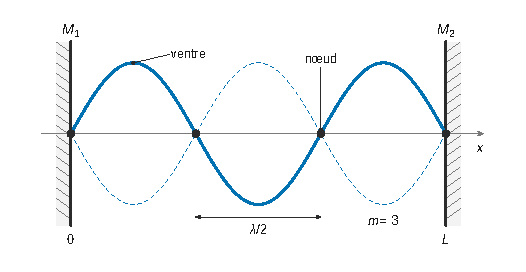
\includegraphics{figures/q19-mode-stationnaire.pdf}
\caption*{Figure 3 --- Mode m = 3 de la cavité sans pertes : un nœud de champ
électrique sur chaque miroir, d'où L = mλ/2}
\end{figure}

\hypertarget{ii-cavituxe9-avec-pertes}{%
\subsection{II --- Cavité avec pertes}\label{ii-cavituxe9-avec-pertes}}

\textbf{Q20.} \(R+T=1\) équivaut à \(I_r+I_t=I_i\) : la puissance incidente se répartit intégralement entre ondes réfléchie et transmise. \textbf{C'est la conservation de l'énergie sur le miroir, supposé sans absorption ni diffusion.}

\textbf{Q21.} Considérons l'onde qui part vers la droite, juste à droite de \(M_1\). Par linéarité, elle est la superposition de deux contributions :

\begin{itemize}
\tightlist
\item
  la \textbf{fraction transmise} à travers \(M_1\) de l'onde de pompe incidente par la gauche, \(\tau\underline E_p\) ;
\item
  la \textbf{fraction réfléchie} sur la face interne de \(M_1\) de l'onde intracavité \(\underline E_G\) qui revient de \(M_2\), soit \(r\underline E_G\) (\(r\) ne dépend pas du sens de traversée).
\end{itemize}

D'où \(\underline E_D=\tau\underline E_p+r\underline E_G\).

\textbf{Q22.} Dans la cavité, \(\underline{\vec E}=\left(\underline E_De^{-jkx}+\underline E_Ge^{jkx}\right)e^{j\omega t}\vec u_y\) (amplitudes définies en \(x=0\)). \(M_2\) est un conducteur parfait : le champ tangentiel est nul en \(x=L\), soit

\equationajustee{\underline E_De^{-jkL}+\underline E_Ge^{jkL}=0}

donc

\equationajustee{\boxed{\underline E_G=-\underline E_D\,e^{-2jkL}}}

(déphasage d'aller-retour \(2kL\) et coefficient de réflexion \(-1\) sur le conducteur parfait).

\textbf{Q23.} \(\underline E_D=\tau\underline E_p-r\underline E_De^{-2jkL}\), et avec \(r=-\sqrt R\), \(\tau=\sqrt{1-R}\) :

\equationajustee{\boxed{\frac{\underline E_D}{\underline E_p}=\frac{\sqrt{1-R}}{1-\sqrt R\,e^{-2jkL}}}}

(dénominateur jamais nul puisque \(\sqrt R<1\)).

\textbf{Q24.} Les deux ondes se propagent dans le vide, donc \(I\propto\lvert\underline E\rvert^2\) avec le même coefficient :

\equationajustee{\begin{aligned}
\left\lvert1-\sqrt Re^{-2jkL}\right\rvert^2&=1+R-2\sqrt R\cos2kL\\
&=(1-\sqrt R)^2+4\sqrt R\sin^2kL
\end{aligned}}

\equationajustee{\frac{I_D}{I_p}=\frac{1-R}{(1-\sqrt R)^2}\cdot\frac{1}{1+\dfrac{4\sqrt R}{(1-\sqrt R)^2}\sin^2kL}}

\equationajustee{\boxed{\begin{aligned}
g&=\frac{1-R}{(1-\sqrt R)^2}\\
&=\frac{1+\sqrt R}{1-\sqrt R}
\end{aligned}}}

\textbf{Q25.} Pour \(R=0{,}960\) :

\equationajustee{\begin{aligned}
\sqrt R&=0{,}9798\\
g&=97{,}99\approx98\\
\mathcal M&=\frac{4\sqrt R}{(1-\sqrt R)^2}\\
&=9{,}60\times10^{3}
\end{aligned}}

Le rapport s'écrit \(I_D/I_p=g/(1+\mathcal M\sin^2kL)\).

\begin{itemize}
\tightlist
\item
  Il vaut \(g\approx98\) quand \(\sin kL=0\).
\item
  Il tombe à \(g/(1+\mathcal M)\approx1{,}0\times10^{-2}\) quand \(\lvert\sin kL\rvert=1\), soit \(10^{-4}\) fois le maximum.
\item
  Il passe sous \(g/2\) dès que \(\lvert\sin kL\rvert>1/\sqrt{\mathcal M}=1{,}0\times10^{-2}\). Il vaut \(2\times10^{-2}\) pour \(\sin^2kL=\frac12\).
\end{itemize}

Il est donc \textbf{négligeable devant son maximum sauf au voisinage immédiat de}

\equationajustee{\boxed{k=\frac{m\pi}{L},\quad m\in\mathbb N^*}}

\textbf{Q26.} La fonction est \(\pi\)-périodique en \(kL\) (fonction d'Airy). Elle présente des pics étroits de hauteur \(g\approx98\), centrés en \(kL=m\pi\).

Leur largeur totale à mi-hauteur vaut \(\Delta(kL)=2/\sqrt{\mathcal M}\approx2{,}0\times10^{-2}\) rad (0,65 \% de la période).

Entre les pics, le fond est quasi nul, de minimum \(1/g\approx10^{-2}\) en \(kL=\pi/2+m\pi\).

\begin{figure}[H]
\centering
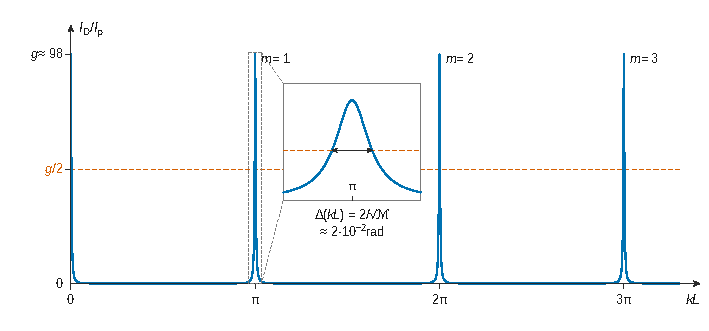
\includegraphics{figures/q26-fonction-airy.pdf}
\caption*{Figure 4 --- Rapport I\_D/I\_p en fonction de kL pour R = 96 \% : pics
de hauteur g ≈ 98 en kL = mπ, de largeur à mi-hauteur 2/√ℳ ≈ 2·10⁻² rad
(zoom), fond quasi nul}
\end{figure}

\textbf{Q27.} Les modes sont les maxima \(k_m=m\pi/L\) ; avec \(\nu=ck/2\pi\) :

\equationajustee{\boxed{\begin{aligned}
\nu_m&=m\frac{c}{2L}\\
\mathrm{FSR}'_\nu&=\frac{c}{2L}\\
&={\mathrm{FSR}}_\nu
\end{aligned}}}

Les modes ont les mêmes fréquences et le même intervalle spectral libre que sans pertes : c'est la même condition d'accord de phase sur un aller-retour, \(2kL=2m\pi\). La différence est qualitative. Sans pertes, seules les fréquences \(\nu_m\) existent. Avec pertes, toute fréquence pénètre un peu, mais efficacement seulement dans des résonances de largeur finie \(\Delta\nu_c\) autour des \(\nu_m\).

\textbf{Q28.} La mi-hauteur correspond à \(\mathcal M\sin^2kL=1\). Près d'un pic, on pose \(kL=m\pi+\delta\), avec \(\lvert\delta\rvert\ll1\) (ici \(1/\sqrt{\mathcal M}\approx10^{-2}\)).

Alors \(\delta_{1/2}=\pm1/\sqrt{\mathcal M}\), d'où \(\Delta(kL)=2/\sqrt{\mathcal M}\).

Comme \(kL=\pi\nu/\mathrm{FSR}'_\nu\) (relation linéaire), \(\Delta(kL)=\pi\Delta\nu_c/\mathrm{FSR}'_\nu\) et

\equationajustee{\boxed{\begin{aligned}
\mathcal F&=\frac{\pi}{\Delta(kL)}\\
&=\frac{\pi\sqrt{\mathcal M}}{2}\\
&=\frac{\pi R^{1/4}}{1-\sqrt R}
\end{aligned}}}

Application numérique : \(\mathcal F=\dfrac{\pi\times0{,}98985}{0{,}020204}\), soit

\equationajustee{\boxed{\mathcal F\approx1{,}54\times10^{2}}}

ce qui confirme \(\Delta\nu_c\ll\mathrm{FSR}'_\nu\).

\textbf{Q29.} À intervalle spectral libre donné, une grande finesse donne une raie très fine, \(\Delta\nu_c={\mathrm{FSR}}_\nu/\mathcal F\). Elle donne donc une \textbf{grande longueur de cohérence} \(\ell_c\approx c/\Delta\nu_c=2L\mathcal F\). On peut alors faire interférer des ondes avec de grandes différences de marche sans perte de contraste (interférométrie à long bras, métrologie des longueurs, détection de très petits déplacements).

\hypertarget{partie-c-milieu-amplificateur-dun-laser}{%
\section{Partie C --- Milieu amplificateur d'un laser}\label{partie-c-milieu-amplificateur-dun-laser}}

\hypertarget{i-uxe9volution-de-populations}{%
\subsection{I --- Évolution de populations}\label{i-uxe9volution-de-populations}}

\textbf{Q30.} Chaque processus est d'ordre 1 par rapport à l'espèce qui disparaît :

\equationajustee{\boxed{\begin{aligned}
v_{\mathrm{pomp}}&=\Gamma n_1\\
v_{\mathrm{nr}}&=k_{\mathrm{nr}}n_3\\
v_{\mathrm{abs}}&=\beta n_1\\
v_{\mathrm{stim}}&=\beta n_2\\
v_{\mathrm{spont}}&=An_2
\end{aligned}}}

\textbf{Q31.} \(\mathrm M\) est consommé par le pompage (\(-\Gamma n_1\)) et l'absorption (\(-\beta n_1\)). Il est produit par l'émission spontanée (\(+An_2\)) et l'émission stimulée (\(+\beta n_2\)). Il n'intervient pas dans la désexcitation non radiative. La somme algébrique donne

\equationajustee{\frac{\mathrm dn_1}{\mathrm dt}=-\Gamma n_1+An_2+\beta n_2-\beta n_1}

\textbf{Q32.} \(\mathrm M^*\) est produit par la désexcitation non radiative et l'absorption, consommé par les émissions stimulée et spontanée. \(\mathrm M^{**}\) est produit par le pompage et consommé par la désexcitation non radiative :

\equationajustee{\boxed{\begin{aligned}
\frac{\mathrm dn_2}{\mathrm dt}&=k_{\mathrm{nr}}n_3+\beta n_1-\beta n_2-An_2\\
\frac{\mathrm dn_3}{\mathrm dt}&=\Gamma n_1-k_{\mathrm{nr}}n_3
\end{aligned}}}

\textbf{Q33.} La somme des trois équations est nulle, car chacun des termes suivants y figure une fois avec chaque signe :

\equationajustee{\pm\Gamma n_1,\quad\pm\beta n_1,\quad\pm\beta n_2,\quad\pm An_2,\quad\pm k_{\mathrm{nr}}n_3}

Donc \textbf{\(n_1+n_2+n_3\) est constant.} Les processus ne font que redistribuer l'espèce M entre ses trois niveaux : c'est la conservation de la quantité totale de M (concentration totale du milieu).

\textbf{Q34.} En régime stationnaire, \(\mathrm dn_3/\mathrm dt=0\) donne

\equationajustee{n_1=\frac{k_{\mathrm{nr}}}{\Gamma}n_3}

Ensuite, \(\mathrm dn_2/\mathrm dt=0\) donne \(k_{\mathrm{nr}}n_3+\beta n_1=(A+\beta)n_2\), soit \((\Gamma+\beta)n_1=(A+\beta)n_2\). Alors

\equationajustee{\begin{aligned}
\Delta n&=n_2-n_1\\
&=\frac{k_{\mathrm{nr}}n_3}{\Gamma}\left(\frac{\Gamma+\beta}{A+\beta}-1\right)\\
&=\boxed{\frac{k_{\mathrm{nr}}(\Gamma-A)}{\Gamma(A+\beta)}\,n_3}
\end{aligned}}

(la troisième équation est redondante, d'après Q33).

\textbf{Q35.} Les constantes de vitesse sont positives et \(n_3>0\) dès que le pompage agit : \(\Delta n\) a le signe de \(\Gamma-A\).

\equationajustee{\boxed{\Delta n>0\iff\Gamma>A}}

Le pompage (qui alimente \(\mathrm M^*\) via \(\mathrm M^{**}\), la relaxation non radiative étant très rapide) doit remplir le niveau excité plus vite que l'émission spontanée ne le vide. \(\beta\) n'intervient pas dans la condition : l'émission stimulée réduit l'inversion sans pouvoir en changer le signe.

\hypertarget{ii-bilan-de-puissance-uxe9lectromagnuxe9tique-dans-le-milieu-amplificateur}{%
\subsection{II --- Bilan de puissance électromagnétique dans le milieu amplificateur}\label{ii-bilan-de-puissance-uxe9lectromagnuxe9tique-dans-le-milieu-amplificateur}}

\textbf{Q36.} Tous les processus ne contribuent pas au bilan de l'onde laser :

\begin{itemize}
\tightlist
\item
  \textbf{pompage} : énergie apportée par une source extérieure, à une autre fréquence ; ne contribue pas directement ;
\item
  \textbf{désexcitation non radiative} : sans photon, l'énergie part en agitation thermique ; ne contribue pas ;
\item
  \textbf{absorption} : retire des photons \(\hbar\omega\) à l'onde, \textbf{perte} (\(\hbar\omega\beta n_1\) par unité de volume et de temps) ;
\item
  \textbf{émission stimulée} : photons cohérents ajoutés à l'onde, \textbf{gain} (\(\hbar\omega\beta n_2\)) ;
\item
  \textbf{émission spontanée} : photons émis dans toutes les directions, sans relation de phase avec l'onde ; ils n'appartiennent pas au faisceau et l'énergie correspondante, prélevée sur les molécules excitées, est \textbf{perdue pour l'onde laser} (\(\hbar\omega An_2\)).
\end{itemize}

\textbf{Q37.} On fait le bilan sur la tranche \([x,x+\mathrm dx]\) de section \(S\), pendant \(\mathrm dt\). La variation de l'énergie \(u_{\text{\text{ém}}}S\,\mathrm dx\) est la somme de trois termes :

\begin{itemize}
\tightlist
\item
  le flux entrant net, \(-\partial_x\Pi\,S\,\mathrm dx\,\mathrm dt\) ;
\item
  plus le terme d'émission stimulée moins absorption, \(\hbar\omega\beta(n_2-n_1)S\,\mathrm dx\,\mathrm dt\) ;
\item
  moins le terme d'émission spontanée, \(\hbar\omega An_2S\,\mathrm dx\,\mathrm dt\).
\end{itemize}

\equationajustee{\frac{\partial u_{\text{\text{ém}}}}{\partial t}=-\frac{\partial\Pi}{\partial x}+\hbar\omega\beta(n_2-n_1)-\hbar\omega An_2}

Avec \(u_{\text{\text{ém}}}=\Pi/c\) et \(\beta=bu_{\text{\text{ém}}}=b\Pi/c\) :

\equationajustee{\boxed{\frac{\partial\Pi}{\partial x}+\frac1c\frac{\partial\Pi}{\partial t}=\gamma(\omega)\Pi-p(\omega)}}

\equationajustee{\boxed{\begin{aligned}
\gamma(\omega)&=\frac{b\hbar\omega(n_2-n_1)}{c}\\
p(\omega)&=\hbar\omega An_2
\end{aligned}}}

Homogénéité : \(p\) en W·m⁻³ et \(\gamma\) en m⁻¹.

\textbf{Q38.} \(\gamma\Pi=\hbar\omega\beta\Delta n\) et \(p=\hbar\omega An_2\) : la condition s'écrit \(An_2\ll\beta\Delta n\). \textbf{L'émission spontanée, incohérente, isotrope et spectralement large, est négligeable devant le gain net par émission stimulée}, qui produit des photons de même direction, fréquence et phase que l'onde. C'est ce qui garantit une lumière cohérente, directive et monochromatique, c'est-à-dire une lumière laser, et non celle d'une lampe.

\textbf{Q39.} En régime stationnaire, \(\dfrac{\mathrm d\Pi}{\mathrm dx}=\gamma\Pi-p\), équation linéaire à coefficients constants. Avec \(\Pi(0)=\Pi_0\) :

\equationajustee{\Pi(x)=\left(\Pi_0-\frac{p}{\gamma}\right)e^{\gamma x}+\frac{p}{\gamma}}

et, puisque \(p\ll\gamma\Pi\),

\equationajustee{\boxed{\Pi(x)=\Pi_0\,e^{\gamma(\omega)x}}}

\textbf{Q40.} \(\gamma=\dfrac{1}{\Pi}\dfrac{\mathrm d\Pi}{\mathrm dx}\) est le \textbf{coefficient de gain linéique} (en m⁻¹) : sur une longueur \(1/\lvert\gamma\rvert\), l'intensité est multipliée ou divisée par \(e\).

Le préfacteur \(b\hbar\omega/c\) étant positif, \(\gamma\) a le signe de \(\Delta n\) :

\begin{itemize}
\tightlist
\item
  \(\Delta n>0\) (inversion) : \(\gamma>0\), amplification exponentielle, l'émission stimulée l'emporte sur l'absorption ;
\item
  \(\Delta n<0\) (situation ordinaire) : \(\gamma<0\), atténuation exponentielle (loi de Beer-Lambert) ;
\item
  \(\Delta n=0\) : milieu transparent.
\end{itemize}

L'amplification exige donc \(\Delta n>0\), c'est-à-dire, en régime stationnaire, \(\Gamma>A\) (Q35).

\equationajustee{\boxed{\gamma>0\iff\Delta n>0\iff\Gamma>A}}

\hypertarget{iii-considuxe9rations-expuxe9rimentales-pour-un-laser-uxe0-colorant-compact}{%
\subsection{III --- Considérations expérimentales pour un laser à colorant compact}\label{iii-considuxe9rations-expuxe9rimentales-pour-un-laser-uxe0-colorant-compact}}

\textbf{Q41.} La solution absorbe entre 550 et 620 nm (vert-jaune-orangé) ; elle transmet le reste du spectre visible et apparaît de la couleur complémentaire de la lumière absorbée, \textbf{le bleu}, d'où son nom. L'émission laser (figure 6) s'étend de 687 à 704 nm environ, maximum vers 695 nm : \textbf{rouge profond}, à la limite du proche infrarouge. Elle est à plus grande longueur d'onde que la bande d'absorption, comme il se doit (pompage vers des niveaux plus hauts que le niveau émetteur).

\textbf{Q42.} Dans le milieu d'indice \(n\), \(k=n\omega/c\) ; les conditions aux miroirs sont inchangées, donc \(kL=m\pi\) et

\equationajustee{\begin{aligned}
\nu_m&=m\frac{c}{2nL}\\
{\mathrm{FSR}}_\nu&=\frac{c}{2nL}
\end{aligned}}

(le résultat de Q19 avec \(c\to c/n\)). La longueur d'onde dans le vide du mode \(m\) vaut \(\lambda_m=c/\nu_m=2nL/m\), donc

\equationajustee{\begin{aligned}
{\mathrm{FSR}}_\lambda&=\lambda_m-\lambda_{m+1}\\
&=\frac{2nL}{m(m+1)}\\
&\approx\frac{2nL}{m^2}\qquad(m\approx650\gg1)\\
&=\frac{\lambda_m^2}{2nL}
\end{aligned}}

ce qui redonne \(\boxed{{\mathrm{FSR}}_\lambda=\dfrac{\lambda^2}{2nL}}\). De façon équivalente, \(\lvert\mathrm d\lambda\rvert=\dfrac{\lambda^2}{c}\lvert\mathrm d\nu\rvert\) appliqué à \(\mathrm d\nu={\mathrm{FSR}}_\nu\).

\textbf{Q43.} Sur la figure 6, les pics vont du mode 664 (\(\approx687{,}7\) nm) au mode 649 (\(\approx703{,}7\) nm). On en tire \({\mathrm{FSR}}_\lambda\approx16{,}0/15=1{,}07\) nm, en accord avec l'insert (1,02 à 1,08 nm). Avec \({\mathrm{FSR}}_\lambda\approx1{,}06\) nm à \(\lambda\approx695\) nm :

\equationajustee{\begin{aligned}
L&=\frac{\lambda^2}{2n\,{\mathrm{FSR}}_\lambda}\\
&=\frac{(695\times10^{-9})^2}{2\times1{,}3587\times1{,}06\times10^{-9}}
\end{aligned}}

\equationajustee{\boxed{L\approx1{,}7\times10^{-4}\ \mathrm m=0{,}17\ \mathrm{mm}}}

Contrôle par le numéro de mode : \(L=m\lambda_m/(2n)=657\times695\times10^{-9}/(2\times1{,}3587)=1{,}68\times10^{-4}\) m. La cavité est bien infra-millimétrique.

\textbf{Q44.} De \(\nu=c/\lambda\), on tire \(\lvert\Delta\nu\rvert=\dfrac{c}{\lambda^2}\lvert\Delta\lambda\rvert\) pour \(\Delta\lambda\ll\lambda\) (ici \(1{,}5\times10^{-3}\) et \(1{,}4\times10^{-4}\) en valeur relative).

Le facteur \(c/\lambda^2\) est le même pour l'intervalle entre modes voisins et pour la largeur d'un pic, pris à la même longueur d'onde :

\equationajustee{\begin{aligned}
\mathcal F&=\frac{{\mathrm{FSR}}_\nu}{\Delta\nu_c}\\
&=\frac{(c/\lambda^2)\,{\mathrm{FSR}}_\lambda}{(c/\lambda^2)\,\Delta\lambda_c}\\
&=\boxed{\frac{{\mathrm{FSR}}_\lambda}{\Delta\lambda_c}}
\end{aligned}}

Application numérique : \(\mathcal F\approx1{,}06/0{,}1\), soit

\equationajustee{\boxed{\mathcal F\sim10}}

C'est environ quinze fois moins que la cavité de la partie B.

\textbf{Q45.} Les pics sont en \(\lambda_m=2nL/m\), espacés de \({\mathrm{FSR}}_\lambda=\lambda^2/(2nL)\). Dans ces relations, \(m\) est entier et \(L\) fixé par la géométrie : le paramètre sensible est \textbf{l'indice optique \(n\) de la solution qui remplit la cavité}. Il dépend de la température (via la masse volumique du liquide) et de la composition chimique (solvant, espèces dissoutes).

On mesure le déplacement des pics, \(\delta\lambda_m/\lambda_m=\delta n/n\). Un déplacement de 0,1 nm correspond à \(\delta n/n\approx1{,}4\times10^{-4}\).

\textbf{Q46.} \emph{Hypothèses.} Miroirs inchangés, donc finesse \(\mathcal F\approx10\) inchangée. Colorant inchangé, donc même bande de gain, de largeur \(\Delta\lambda_{\mathrm{gain}}\approx15\text{–}20\) nm autour de 695 nm. Seule \(L\) passe de 0,17 mm à \(L\approx1\) m.

\emph{Chiffrage.} Avec la cavité remplie de colorant (\(n=1{,}3587\)) :

\equationajustee{\begin{aligned}
{\mathrm{FSR}}_\lambda&=\frac{\lambda^2}{2nL}\\
&=\frac{(695\times10^{-9})^2}{2\times1{,}3587\times1}\\
&=1{,}8\times10^{-13}\ \mathrm m\\
&=1{,}8\times10^{-4}\ \mathrm{nm}
\end{aligned}}

\equationajustee{\begin{aligned}
{\mathrm{FSR}}_\nu&=\frac{c}{2nL}\\
&=110\ \mathrm{MHz}
\end{aligned}}

Pour une cavité essentiellement dans l'air (\(n\approx1\)), on trouverait \(2{,}4\times10^{-4}\) nm : même conclusion. On en déduit :

\begin{itemize}
\tightlist
\item
  nombre de modes dans la bande de gain : \(N\approx\Delta\lambda_{\mathrm{gain}}/{\mathrm{FSR}}_\lambda\approx10^{5}\) ;
\item
  largeur de chaque résonance : \({\mathrm{FSR}}_\lambda/\mathcal F\approx2\times10^{-5}\) nm ;
\item
  numéro de mode : \(m=2nL/\lambda\approx4\times10^{6}\).
\end{itemize}

\emph{Allure.} Un spectromètre usuel résout \(10^{-2}\) à \(10^{-1}\) nm, soit 50 à 500 fois l'écart entre modes : les modes ne sont pas résolus. Le spectre observé est une \textbf{bande quasi continue} dont l'enveloppe est la courbe de gain du colorant (même position et même largeur, environ 687--704 nm), au lieu du peigne de seize pics bien séparés de la figure 6.

\begin{figure}[H]
\centering
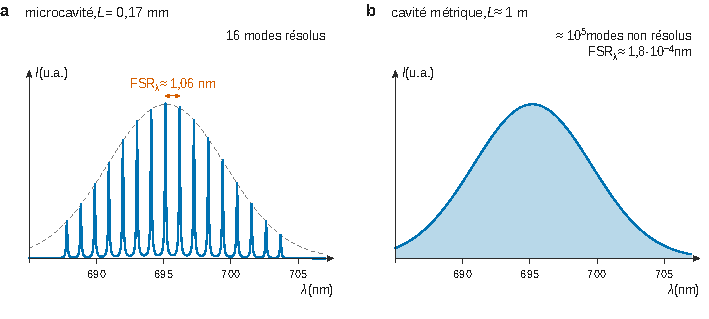
\includegraphics{figures/q46-spectres-cavite-courte-longue.pdf}
\caption*{Figure 5 --- Allure des spectres à colorant et miroirs identiques : (a)
microcavité, 16 modes séparés de 1,06 nm ; (b) cavité métrique, environ
10⁵ modes non résolus, bande continue sous la courbe de gain}
\end{figure}

\emph{Commentaire.} Plus la cavité est longue, plus les modes sont serrés : la microcavité sélectionne naturellement une quinzaine de modes séparés, ce qui permet d'en suivre le déplacement (capteur, Q45). Un laser à cavité métrique est fortement multimode (la compétition entre modes limite le nombre de modes effectivement oscillants sans rendre le spectre résoluble) ; pour le rendre monomode et accordable, on insère des éléments sélectifs (réseau, étalon Fabry-Pérot, filtre biréfringent). En contrepartie, il offre un plus grand volume amplificateur et donc davantage de puissance.

\end{document}
